\section{Core concepts}\label{sec:core-concepts}

In this section, we discuss the integral core concepts of Continuous Integration
in order to give the reader a good understanding of its principles.

\subsection{Motivation}\label{sec:motivation}

The main goal of Continuous Integration is to minimize integration issues when
deploying release-versions of the product. Because builds happen often and
regularly, these issues can be identified very quickly and will not cause
stressful last-minute fixes. The incorporation of unit tests into the
build (see \ref{sec:tests}) can further increase fast error detection. Another
important aspect of Continuous Integration is the provision of a reporting
agent, a way that developers get informed about failing builds.

\subsubsection{Merge hell}

In big software projects, a large number of developers work together to create
software. To be able to work on the same project simultaneously, typically, a
version-control system such as GIT is utilized
\footnote{\url{http://git-scm.com/}}.\\

Developers usually branch off from a common baseline ("master"), implement their
feature in their own copy ("feature-branch") and when finished, merge their
branch back into the master. However, if a large number of developers do that,
and their features are large and/or implemented in overlapping parts of the
source code, developers have to face merge-conflicts when integrating their
branch back into the baseline. These conflicts can easily get out of hand.
Figure \ref{fig:merge-hell} shows an example of such a situation.

\begin{figure}[h]
    \centering
    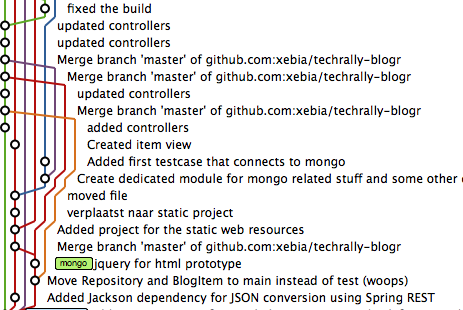
\includegraphics[width=0.6\linewidth]{images/merge-hell.png}
    \caption{An example of "merge-hell" \cite{mooij:2010}}
    \label{fig:merge-hell}
\end{figure}

Solving these conflicts can be non-trivial task, especially for the introduction
of completely new features, since the developer who has to perform the merge
typically is not yet accustomed to the code another developer only just
created.\\

In order to keep large merge conflicts to a minimum and therefore circumvent
this issue, Continuous Integration strives to integrate features back into the
baseline branch frequently (e.g. multiple times per day).  Of course, this means
that the term "feature" is bound to refer only to small changes throughout the
project's life cycle.

\subsubsection{Automation}\label{sec:automation}

It would not be possible to facilitate Continuous Integration without a high
degree of automation present in the building process. The CI-server has to be
able to perform each task (building, running tests, analysis, deployment) at
least mostly automatically, or the concept would not be feasible. It makes sense
cost-wise that the build-server uses the same system developers use locally to
build the product, thus Continuous Integration has to be taken into account when
first designing the project's development architecture.\\

A big build can take time, so Continuous Integration systems have to be smart
about it and for example only recompile source files that actually have changed.

\subsection{Build types \& triggers}\label{sec:build-types-triggers}

Continuous Integration systems usually go beyond the capabilities of a simple
build-server. While running tests is also a main-task for a CI-system, they also
have the capabilities to measure code metrics or perform actual deployment.

\subsubsection{Triggers}\label{sec:triggers}

What triggers these various build types is usually configured in the Continuous
Integration system. The trigger scheme usually falls into one or more of the
following categories:

\begin{itemize}
    \item Manually
    \item Timed
    \item On change
\end{itemize}

The simplest form of trigger is a manual one. It can be used as a fallback when
other triggers are unavailable and can also be utilized for testing the
build-system itself. Continuous Integration systems usually provide this
functionality via a user interface such as a website.\\

For timed builds, a simple time-frame is configured for the build to happen -
e.g. daily, hourly, etc. The Continuous Integration system can employ its own
timing mechanism or rely on frameworks provided by the operating system (e.g.
cronjobs).\\

The most useful type of trigger is a change-based trigger. Here, the Continuous
Integration system listens for changes on the project's source code repository
and only builds the project when an actual change has occurred. This trigger
enables developers to get almost instant feedback for whether their change has
broken the build or not.

The listening itself can be accomplished by a simple polling mechanism, however
the cleanest approach is based on VCS-based hooks. Here, the version-control
system provides a possibility to execute arbitrary commands on certain events,
such as a commit/merge on a specific branch.\\

GIT for example supports both client-side and server-side hooks. Client-side
hooks can be used to do some pre-push checks, but they have to be configured
individually for each developer. The really useful type of git-hook in terms of
Continuous Integration are server-side hooks of which GIT provides 3 types
\cite{chacon:2009}:

\begin{itemize}
    \item pre-receive: Run when handling a push from a client
    \item update: Similar to pre-receive, but run for each branch
    \item post-receive: Runs after the push process has completed. This is
        typically used for triggering a CI-based build.
\end{itemize}

Similar hooking mechanisms are available in other version control systems, such
as
SVN\footnote{\url{http://svnbook.red-bean.com/nightly/en/svn.reposadmin.create.html}}
or Mercurial\footnote{\url{http://mercurial.selenic.com/wiki/Hook}}.\\

Triggers can of course be combined to provide multiple trigger points.


\subsubsection{Builds}\label{sec:builds}

\subsubsection{Tests}\label{sec:tests}

Best practice: Test in clone of real production...

\subsubsection{Static code analysis}\label{sec:static-code-analysis}

\subsubsection{Deployment}\label{sec:deployment}

Address works-for-me-bugs

\paragraph{Migrations}\label{sec:migrations}

\subsection{Source control}\label{sec:source-control}

\subsection{Reporting}\label{sec:reporting}

